\documentclass[a4paper]{article}

%% Language and font encodings
\usepackage[utf8x]{inputenc}
\usepackage[T1]{fontenc}
\usepackage[portuguese]{babel}

%% Sets page size and margins
\usepackage[a4paper,top=3cm,bottom=2cm,left=2cm,right=2cm,marginparwidth=1.75cm]{geometry}

%%tabelas sofisticadas
\usepackage{booktabs}
\usepackage[table,xcdraw]{xcolor}

%% Pacotes úteis
\usepackage{amsmath}
\usepackage{graphicx}
\usepackage{subfigure} %pacote para  subfiguras
\usepackage[colorinlistoftodos]{todonotes}
\usepackage[colorlinks=true]{hyperref}

%% Desenhando circuitos
\usepackage{circuitikz}




\title{Seu primeiro relatório \LaTeX}
\author{Você, Fulano e Beotrano}

\begin{document}
\maketitle

\begin{abstract}
Seu resumo do relatório, resumo não é introdução! Por exemplo, o excerto abaixo foi extraído do relatório de alunos do 1s2017, note que ele resume as atividades desenvolvidas e apresentadas no relatório, porém não faz uma introdução exagerada ao assunto abordado.

"\textit{Calculamos a partir da montagem de circuitos RC e RLC a resistência interna do osciloscópio, bem como os valores de capacitância dos componentes utilizados. Analisamos as curvas dos circuitos passa-altas, passa-baixas e passa banda, juntamente com seus respectivos diagramas de bode, comparando-as com curvas esperadas fornecidas na literatura sobre o assunto. Utilizando um método baseado em assíndotas, estimamos valores para as frequências de ressonância e de corte, comparando-os com valores experimentais e teóricos}"
\end{abstract}

\section{Introdução}

Sua introdução vai aqui! Alguns exemplos de comandos e recursos comumente usados estão listados abaixo, para ajudá-lo a começar. Se você tiver uma pergunta, use o menu de ajuda (``?? '') Na barra superior para procurar ajuda ou nos fazer uma pergunta.
\section{Organização do relatório}
Uma maneira simples de organizar um relatório é seguir as seções enunciadas a seguir (assumindo que o resumo já foi incluído no início do relatório),
\begin{itemize}
\item \textbf{Introdução} -- Descrever o propósito do experimento, as motivações de executá-los e possíveis conceitos físicos que serão explorados.
\item \textbf{Materiais e métodos} -- Listar equipamentos (modelo e número de identificação quando possível) e componentes (valores nominais) utilizados,
\item \textbf{Resultados} -- Apresentar os resultados experimentais, inclua eventuais medidas de caracterização de componente (e.g., resistências, resistência parasítica do indutor). Avalie se é melhor apresentar o dado na forma de tabela ou gráfico. Note que um diagrama de Bode não deve ser apresentado na forma de tabela, enquanto que os valores de resistência utilizados poderiam utilizar este formato de apresentação. 
\begin{itemize}

\item Caso apresente dados que serão usados para ajustar um modelo teórico, aproveite o espaço do gráfico para apresentar o ajuste. Faça uma breve discussão do ajuste,incluindo os parâmetros extraídos e equações utilizadas (evite deduções nesta parte). 

\item Sendo seu experimento constituído de mais de um conjunto de dados, utilize subseções.
\end{itemize}

\item \textbf{Discussão} -- Esta parte poderia ser integrada à seção de resultados, permitindo uma discussão mais direta. Por exemplo, suponha que você fez um ajuste de um modelo teórico aos dados experimentais. Este ajuste  pode ser apresentado diretamente com o gráfico da seção de "Resultados", porém sua discussão ficaria pendende. Portanto
\item \textbf{Referências} -- Esta seção inclui as referências bibliográficas utilizadas no texto. Não economize aqui, coloque todas as referências utilizadas. No \LaTeX isto é muito fácil através do arquivo de referência .bib, o qual se usa com algum programa de gerência de bibliografias, como o Mendeley, Zotero, etc. Estes mesmos programas também são compatíveis com Microsoft Word, OpenOffice, etc.
\end{itemize}

\section{Alguns exemplos para começar}

\subsection{Como incluir figuras}

Primeiro você tem que carregar o arquivo de imagem do seu computador usando o link de upload no menu do projeto. Em seguida, use o comando includegraphics para incluí-lo em seu documento. Use o ambiente de figura eo comando legenda para adicionar um número e uma legenda à sua figura. Veja o código da Figura \ref{fig:frog} nesta seção para um exemplo.

\begin{figure}
\centering
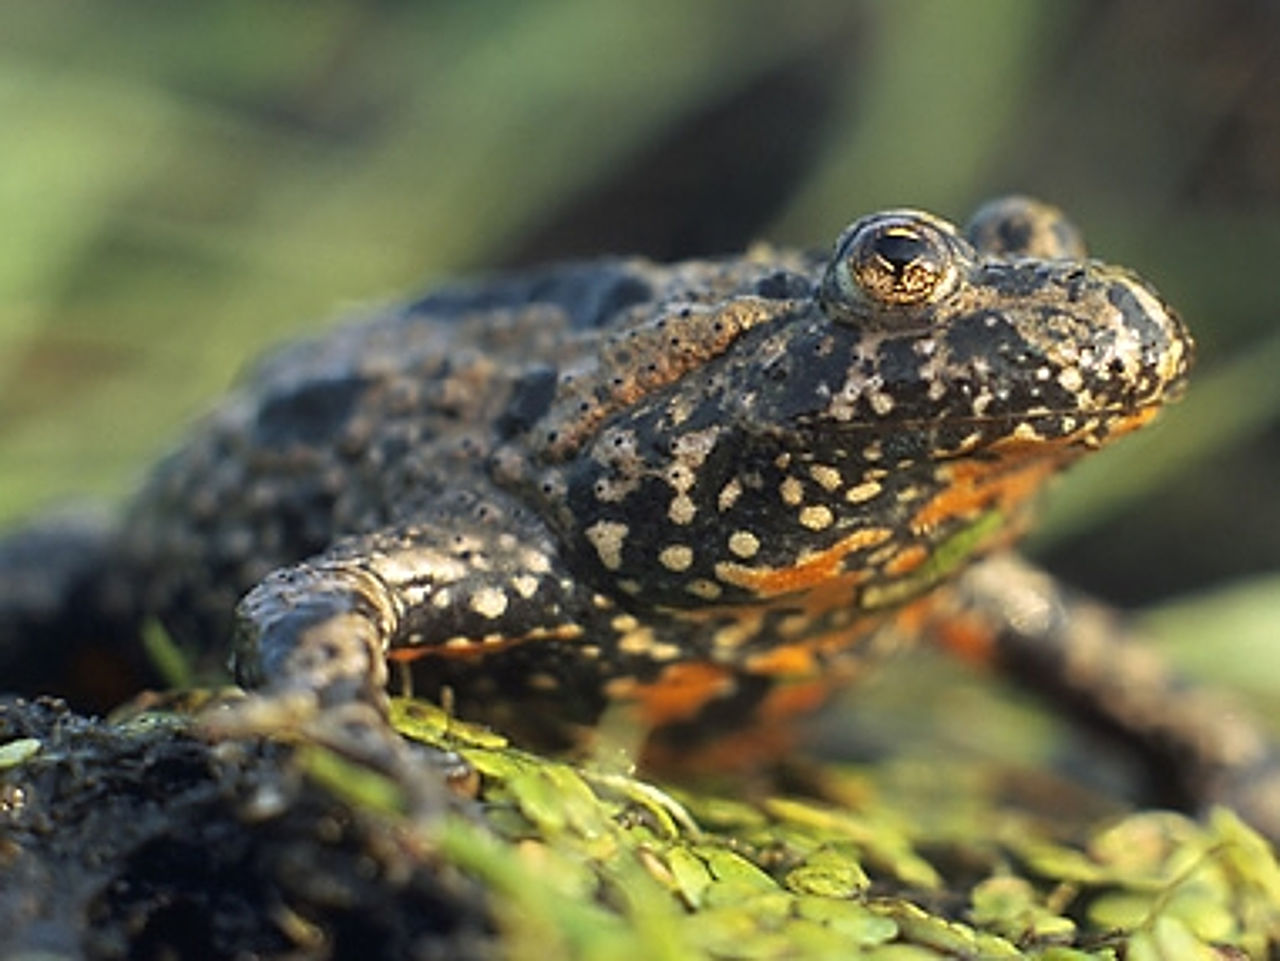
\includegraphics[width=0.3\textwidth]{sapo.jpg}
\caption{\label{fig:frog}Este sapo foi carregado através do menu do projeto. Fotografia extraída da Wikipedia~\cite{wiki:sapinho}}
\end{figure}

\subsection{Como adicionar comentários}

Os comentários podem ser adicionados ao seu projeto clicando no ícone de comentário na barra de ferramentas acima. % * <john.hammersley@gmail.com> 2016-07-03T09:54:16.211Z:
%
%  Exemplo de comentário
%
Para responder a um comentário, basta clicar no botão de resposta no canto inferior direito do comentário e fechá-los quando terminar.

Os comentários também podem ser adicionados às margens do PDF compilado usando o comando todo \todo{Aqui está um comentário na margem!}, Como mostrado no exemplo à direita. Você também pode adicionar comentários inline:

\todo[inline, color=green!40]{Este é um comentário inline. Isto é útil para chamar a atenção dos colegas de grupo para algum ponto do relatório!}

\subsection{Como adicionar tabelas}

Use a tabela e os comandos tabulares para tabelas básicas --- veja Tabela \ref{tab:widgets}, por exemplo. Tabelas mais complicadas também são possível, porém é interessante usar neste caso geradores de tabela, como o site \href{http://www.tablesgenerator.com}.

\begin{table}
\centering
\begin{tabular}{l|r}
Item & Quantity \\\hline
Widgets & 42 \\
Gadgets & 13
\end{tabular}
\caption{\label{tab:widgets}Um exemplo de tabela.}
\end{table}

%-----------
%TABELA
%-----------
\begin{table}
\centering

\begin{tabular}{@{}lllll@{}}
\toprule

\rowcolor[HTML]{BBDAFF} 
Turmas &        & B                                       & C                                        & A,D                             \\ \midrule
Semana &        & Terça                                   & Quarta                                   & Quinta                          \\
       &        &                                         &                                          &                                 \\
1      & 27-Feb & \cellcolor[HTML]{96FFFB}Feriado (28/02) & \cellcolor[HTML]{96FFFB}Feriado (01/03)  & AC/Instrumentos                 \\
2      & 6-Mar  & AC/Instrumentos                         & AC/Instrumentos                          & Aquisição/Python                \\
3      & 13-Mar & Aquisição/Python                        & \cellcolor[HTML]{FFCCC9}Aquisição/Python & \cellcolor[HTML]{FFCCC9}Exp. 1a \\
4      & 20-Mar & Exp. 1a                                 & Exp. 1a                                  & Aula teórica 1                  \\
5      & 27-Mar & Aula teórica 1                          & Aula teórica 1                           & Exp. 1b (T1)                   
\end{tabular}
\caption{Tabela sofisticada criada usando o TableGenerator.}
\label{tab:tabela_bonita}
\end{table}
%-----------
% FIM DA TABELA
%-----------
\subsection{Como escrever Matemática}

\LaTeX{} é demais para formatar matemática. Seja $ X_1, X_2, \ldots, X_n $ uma seqüência de variáveis aleatórias independentes e identicamente distribuídas com $\text{E}[X_i] = \mu$ e $\text{Var}[X_i] = \sigma^2 < \infty$, e 

\[S_n = \frac{X_1 + X_2 + \cdots + X_n}{n}
      = \frac{1}{n}\sum_{i}^{n} X_i\]
denotam sua média. Então, à medida que $ n $ se aproxima do infinito, as variáveis aleatórias $\sqrt{n}(S_n - \mu)$ convergem para a distribuição  Normal $\mathcal{N} (0, \sigma^2) $.


\subsection{Como criar Seções e Subsecções}

Use a seção e subseções para organizar seu documento. Basta usar os botões de seção e subseção na barra de ferramentas para criá-los, e vamos lidar com todos os formatação e numeração automaticamente.

\subsection{Como adicionar Listas}

Você pode fazer listas com numeração automática \dots

\begin{enumerate}
\item Like this,
\item and like this.
\end{enumerate}
\dots or bullet points \dots
\begin{itemize}
\item Like this,
\item and like this.
\end{itemize}

\subsection{Como desenhar circuitos usando o Tikz}
Um exemplo de circuito de duas portas é mostrado na fig. \ref{fig:circuitoRC}. Também é possível montar uma figura com subfiguras, como na fig. \ref{fig:circuitos}.
%-----------
% FIGURA
%-----------
\begin{figure}
\centering
\begin{circuitikz}[scale=1]
		\node (Xi) at (0.7,0.7) {$V_1$};
		\node (Xf) at (3.7,0.7) {$V_2$};
		\draw [semithick,->] (Xi) -- (0.1,0.1);
		\draw [semithick,->] (Xf) -- (3.1,0.1);
		\draw to [resistor, o-o, l_=$R$] ++(2,0)
			(2,0) to [short,o-o] ++(1,0)
			(2,0) to [capacitor, o-o, l=$C$] ++(0,-2)
			node[ground] {};
\end{circuitikz}
\caption{Circuito RC desenhado usando o pacote CircuitTikz}
\label{fig:circuitoRC}
\end{figure}
%-----------
% FIM DA FIGURA
%-----------

%-----------
% FIGURA
%-----------
\begin{figure}
\centering
%% CIRCUITO 1, subfigura 1
\subfigure[\label{fig:rc_pa}Passa-altas RC]{
\begin{circuitikz}[scale=1]
		\node (Xi) at (0.7,0.7) {$V_1$};
		\node (Xf) at (3.7,0.7) {$V_2$};
		\draw [semithick,->] (Xi) -- (0.1,0.1);
		\draw [semithick,->] (Xf) -- (3.1,0.1);
		\draw to [resistor, o-o, l_=$R$] ++(2,0)
			(2,0) to [short,o-o] ++(1,0)
			(2,0) to [capacitor, o-o, l=$C$] ++(0,-2)
			node[ground] {};
\end{circuitikz}
}
%% CIRCUITO 2, subfigura 1
\subfigure[\label{fig:rc_pb}Passa-baixas RC]{
\begin{circuitikz}[scale=1]
		\node (Xi) at (0.7,0.7) {$V_1$};
		\node (Xf) at (3.7,0.7) {$V_2$};
		\draw [semithick,->] (Xi) -- (0.1,0.1);
		\draw [semithick,->] (Xf) -- (3.1,0.1);
		\draw to [capacitor, o-o, l_=$C$] ++(2,0)
			(2,0) to [short,o-o] ++(1,0)
			(2,0) to [resistor, o-o, l=$R$] ++(0,-2)
			node[ground] {};
\end{circuitikz}
}
%% CIRCUITO 3, subfigura 3
\subfigure[\label{fig:rl_pa}Passa-altas RL]{
\begin{circuitikz}[scale=1]
		\node (Xi) at (0.7,0.7) {$V_1$};
		\node (Xf) at (3.7,0.7) {$V_2$};
		\draw [semithick,->] (Xi) -- (0.1,0.1);
		\draw [semithick,->] (Xf) -- (3.1,0.1);
		\draw to [resistor, o-o, l_=$R$] ++(2,0)
			(2,0) to [short,o-o] ++(1,0)
			(2,0) to [inductor, o-o, l=$L$] ++(0,-2)
			node[ground] {};
\end{circuitikz}
}
\caption{Possíveis configurações de filtros baseados em circuitos RC e RL. A tensão $V_1$ é denominada tensão de entrada, $V_2$ é denominada tensão de saída; ambas serão medidas no osciloscópio.}
\label{fig:circuitos}
\end{figure}
%-----------
% FIM DA FIGURA
%-----------

\subsection{Como adicionar citações e uma lista de referências}

Você pode carregar um arquivo \verb|.bib| contendo suas entradas BibTeX, criado com JabRef; Ou importar sua biblioteca \href{https://www.overleaf.com/blog/184}{Mendeley}, CiteULike ou Zotero como um arquivo \verb|.bib|. Você pode então citar entradas dele, assim: \cite{Born:1969aa}, ou \cite{WalHalRes08}. Lembre-se de especificar um estilo bibliográfico, bem como o nome do arquivo \verb|.bib|. 

Existe um tutorial (em inglês) \href{https://www.overleaf.com/help/97-how-to-include-a-bibliography-using-bibtex}{tutorial aqui} to learn more about BibTeX.

We hope you find Overleaf useful, and please let us know if you have any feedback using the help menu above --- or use the contact form at \url{https://www.overleaf.com/contact}!

%-----------
% BIBLIOGRAFIA
%-----------
\bibliographystyle{alpha}
\bibliography{Mendeley_F429} % edite este arquivo no Mendeley, ou crie sua própria biblioteca Mendeley.

\end{document}